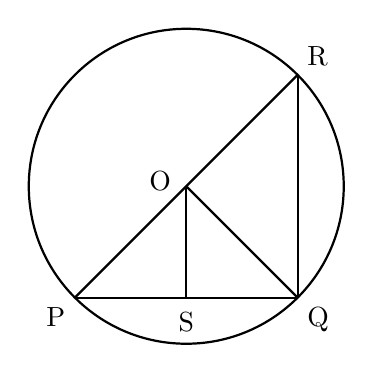
\begin{tikzpicture}[scale=1]

    % Define the radius of the circle
    \def\R{2}

    % Define the center of the circle
    \coordinate (O) at (0,0);

    % Define the points on the circle based on the geometric properties shown in the image
    % P, O, R form a straight line (diameter). 
    % R is approximately at 45 degrees, making P at 225 degrees.
    % Q is horizontally aligned with P and vertically aligned with R, making it 315 degrees.
    \coordinate (R) at (45:\R);
    \coordinate (P) at (225:\R);
    \coordinate (Q) at (315:\R);

    % S is the intersection of the perpendicular from O to PQ, which makes it the midpoint of PQ
    \path (P) -- (Q) coordinate[midway] (S);

    % Draw the circle
    \draw[thick] (O) circle (\R);

    % Draw the main line segments
    \draw[thick] (P) -- (R); % Diameter connecting P and R through O
    \draw[thick] (P) -- (Q); % Chord PQ
    \draw[thick] (R) -- (Q); % Chord RQ
    \draw[thick] (O) -- (S); % Line segment from center O to S
    \draw[thick] (O) -- (Q); % Radius from center O to Q

    % Add the labels for each point exactly as shown in the image
    \node[above right] at (R) {R};
    \node[below left] at (P) {P};
    \node[below right] at (Q) {Q};
    \node[below, yshift=-2pt] at (S) {S};
    
    % Position O slightly to the left of the center to match the reference image
    \node[left, xshift=-2pt, yshift=2pt] at (O) {O};

\end{tikzpicture}